\subsection{Relevant Technologies}
% compare the available technologies and propose how to apply them to our system

\subsubsection{Sensor Ranging}
% Toby - sensors, haptics basic goal
\noindent Ranging sensors are used to provide distance-to-obstacle information for a plethora of products today. They are popularly found in robotics, where they are able to provide awareness of the surroundings, vehicles, where they enable autonomous navigation, or for smart facility and home solutions, where they detect movement and are used to trigger various actions. FORWARD requires sensors to enable safe navigation and it is thus appropriate to examine the technologies available to determine which to install on the walker. The intent also is two-fold in that it is desired to gain knowledge of what is attainable, namely what information about the surroundings can we provide our processor and how accurate and insightful can that information be. Note that, FORWARD does not implement features of user health status or tracking and so we do not examine GPS as a relevant technology. FORWARD navigates autonomously, and it will do this by use of \textbf{\textit{time-of-flight sensing}}.\\

\noindent \underline{\textit{Ultrasonic}} There are differing variations of ultrasonic sensing technology, mainly varying by their 1) transmitting and receiving hardware, which can be realized as mono or multistatic, 2) emission and detection capability, which stipulates their active or passive status, and 3) their operating frequency \cite{sonar-type}. As far as whether the hardware comes in the form of a multistatic setup or a single transceiver (emits and receives ultrasound), FORWARD's requirements do not necessarily rule out one or the other. Monostatic could be slightly more conducive to mounting on the walker legs and help retain a lower profile because of their smaller (2x) dimensions.\\

\begin{figure}[H]
	\centering
	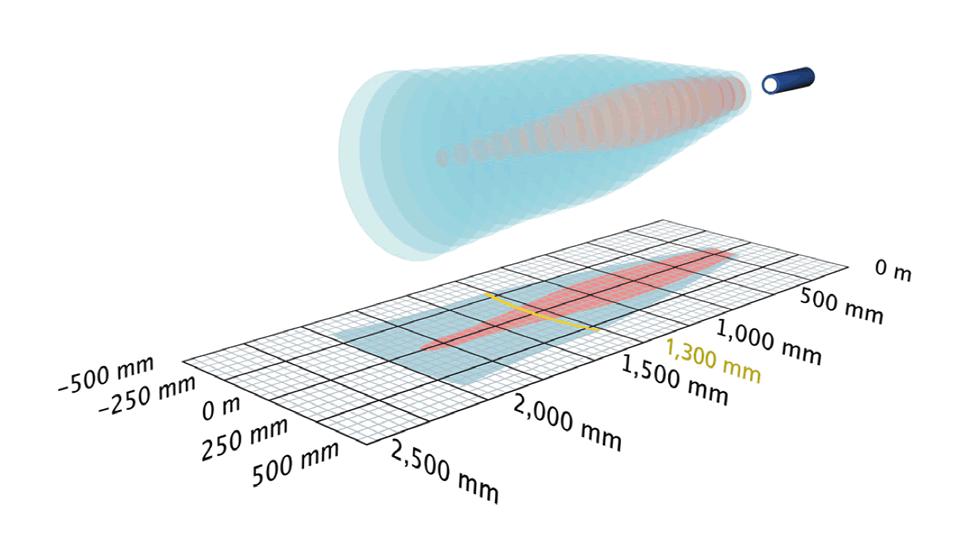
\includegraphics[width=0.7\textwidth]{./Images/cool-ultrasonic-directivity.png}
	\caption{\label{fig:cool-directivity}Ultrasonic Directivity \cite{coolUltraDirect}}
\end{figure}

\noindent \underline{\textit{LiDAR}} We deploy LiDAR in the context of this project as 1) oriented laterally, 2) topographic, and 3) scanning method: rotating, fixed (solid-state), flash \cite{lidar-type}. As designers, we must also consider that LiDAR reliability may be affected by the reflectivity of the target objects and ambient lighting of the surroundings. This is one of the primary reasons both sound and light sensing applications are under consideration. Note, figure \ref{fig:lidarazimuth} shows a scanning LiDAR. In this project, the azimuth and elevation difference are both negligible, as the light beam is single-point. Scanning would require another subsystem with servomotors, which is not in specification or budget.\\

\begin{figure}[H]
	\centering
	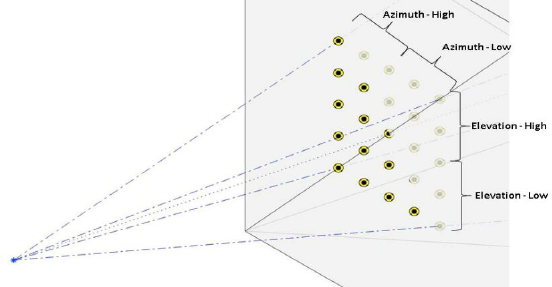
\includegraphics[width=0.7\textwidth]{./Images/FOV-scanning-LIDAR.png}
	\caption{\label{fig:lidarazimuth}Scanning LiDAR FOV \cite{coolLiDARfov}}
\end{figure}

% advanced goal
\subsubsection{Walker Stability} \label{sssec:3_2stability}
\noindent \underline{\textit{Inertial Measurement}} Units are comprised of a magnetometer and accelerometer, which obtain the acceleration and body rate readings of the walker. This is traditionally done by a reading a gyroscope rotation or looking at the magnetic field. It could be greatly beneficial to gain this data, not only for analytical use, but for functionality. Some of the stretch requirements include curb lifting, fall prevention, and incline decline adaptation. With an IMU on-board, the walker can respond appropriately to each scenario. For instance, when lifting over a curve, there can be a certain pitch angle limit imposed to prevent tipover. This is expanded in a similar fashion for fall prevention, where if the user leans too much on the handlebars and causes a tipover, the IMU data can inform the motors of a decision. Finally, the IMU angles are also useful when traversing over inclines or declines. The body rates may be useful for stability while turning, smoothing the roll.\\

% stretch goal
\noindent \underline{\textit{CV Depth Perception}} Computer vision will prove to be outstanding for articially intelligent object identification and hazard classification, but it also help aid in ranging given the trade-off of a higher price point and more heavy computation.\\

\noindent \underline{\textit{Sonar vs. LiDAR for Detection}} As gleaned from \cite{sonar-vs-lidar}, ultrasonic sensors are advantageous for their low cost, simple digital input and output, and wider FOV. However, they lack in their exposure to environment, slower response time, and larger physical size. LiDAR sensors on the other hand, are small and lightweight, and have a fast response time. However, they generally cost more and have a more narrow FOV because of their environmental seal and laser physics.\\

\noindent \underline{\textit{Balanced Sensor Informants}} When comparing the selling points of cameras and traditional sensing methods, we see that each have their advantages. Cameras allow for the most detailed information about the shape and size of the obstacle, but they rely on a lens that can become dirty. The camera may also not operate well in lowlight environments. By still including the ultrasonic and LiDAR, FORWARD can always sense obstacles and have multiple informants. Each sensing method covers the next. When ultrasonic may be affected by wind, the LiDAR is not. When the reflectivity of an object may obscure the LiDAR, the sound waves can still detect. \cite{camera-vs-sensor}.\\

\noindent \underline{\textit{Sensor Fusion}} Implementation of sensor fusion to converge on a most accurate range solution would not be beneficial derived from the ultrasonic and LiDAR outputs, because they should both give nearly identical readings, and thus, leaving no need for fusion. However, it could greatly enhance the computer vision by allowing it to not only identify and classify hazards, but also aid with range detection. The range given by the camera's depth perception could be fused with the more reliable range readings from the front of the walker to further confirm the presence and distance of obstacles. Additionally, the camera could inform the avoidance subsystem of ultrasonic and LiDAR range data to for any reason, ignore.\\

% Matthew - MCU, computer vision, audio



% Morgan - Power supply, motors, motor shield, steering, braking